
\section{Introduction}
\label{sec:Intro}

Language and compiler designers are well aware of the intricacies of erased generics \cite{leroy-unboxed-objects, morrison-napier88, harper-intensional-type-analysis, java-erasure, dot-net-generics, iuli-thesis, miniboxing, spj-unboxed-values}, one of which is requiring object-based representations for primitive types. To illustrate this, let us analyze the |identity| method, parameterized on the argument type, |T|:

\begin{lstlisting-nobreak}
 def identity[`T`](arg: `T`): `T` = arg
 val x: Int = identity[Int](5)
\end{lstlisting-nobreak}

The low-level compiled code for |identity| needs to handle incoming arguments of different sizes and semantics: booleans, bytes, characters, integers, floating point numbers and references to heap-allocated objects. To implement this, some compilers impose a uniform representation, usually based on references to heap objects. This means that primitive types, such as integers, have to be represented as objects when passed to generic methods. The process of representing primitive types as objects is called boxing. Since boxing slows down execution, whenever primitive types are used outside generic environments, they use their stack-based (unboxed) representation. Thus, in the low-level compiled code, |x| is using the unboxed representation, denoted as |int|:

\begin{lstlisting-nobreak}
 def identity(arg: `Object`): `Object` = arg
 // val x: Int = identity[Int](5):
 val arg_boxed: `Object` = box(5)
 val ret_boxed: `Object` = identity(arg_boxed)
 val x: `int` = unbox(ret_boxed)
\end{lstlisting-nobreak}

The low-level code shows the two representations of the high-level |Int| concept: the unboxed primitive |int| and the boxed |Object|, which is compatible with erased generics. There are two approaches to exposing this duality in programming languages: In Java, both representations are accessible to programmers, making them responsible for the choice and exposing the language feature interactions. On the other hand, in order to avoid burdening programmers with implementation details, languages such as ML, Haskell and Scala expose a unified concept, regardless of its representation. Then, during compilation, the representation is automatically chosen based on the interaction with the other language features and the necessary coercions between representations, such as |box| and |unbox|, are added to the code.

This strategy of exposing a unified high-level concept with multiple representations is used in other language features as well:

\textbf{Value classes} \cite{gosling-value-classes, dot-net-value-types-www, scala-value-classes-sip} behave as classes in the object-oriented hierarchy, but are optimized to efficient C-like structures \cite{cxx-stroustrup} where possible. This exposes two representations of the value class concept: an inline, efficient struct representation and a flexible object-oriented representation that supports subtyping and virtual method calls.

\textbf{Specialization} \cite{specialization-iuli, iuli-thesis, goetz-specialization} is an optimized translation for generics, which compiles methods and classes to multiple variants, each adapted for a primitive type. An improvement to specialization is using the miniboxed representation \cite{miniboxing, miniboxing-www}, which creates a single variant for all primitive types, called a minibox. In this transformation, a generic type |T| can be either boxed or miniboxed, in yet another instance of a concept with multiple representations.

\textbf{Multi-stage programming} (also referred to as ``staging'') \cite{taha-intro} allows executing a program in multiple stages, at each execution stage generating a new program that is compiled and run, until the final program outputs the result. In practice, this technique is used to lift expressions to operation graphs and to generate new, optimized code for them. This shows a very different case of dual representations: a value can be represented either as itself or as a lifted expression, to be evaluated in a future execution stage.

The examples above seem like unrelated language features. And, indeed, compiler implementers have provided dedicated solutions for each of them, entangling the core transformation mechanism with assumptions about the language and platform. For instance, the solutions employed by ML and Scala are aimed at satisfying the constraints of erased generics \cite{java-erasure, leroy-unboxed-objects, thiemann-unboxed-objects-cps}, and hardcode this decision into their rewriting algorithm. Miniboxing uses a custom transformation implemented as a Scala compiler plugin \cite{miniboxing, miniboxing-www}, aimed at only the miniboxed representation. Finally, the Lightweight Modular Staging framework \cite{tiark-lms} in Scala relies on a custom fork of the main compiler, dubbed Scala-Virtualized \cite{scala-virtualized}, which is specifically retrofitted to support lifting language constructs.

Yet, these transformations share two common traits:\\ (1) the use of multiple representations for the same concept and (2) the automatic introduction of coercions between these representations during program compilation. These similarities suggest there is an underlying principle that generalizes the individual algorithms. We believe exposing this principle can disentangle the transformations from their assumptions, providing a framework that researchers can formally reason about and that implementors can reuse when developing new transformations.

To this end, we present an elegant and minimalistic type-driven mechanism that uses annotations to guide the introduction of coercions between alternative representations, which we call the Late Data Layout (LDL) mechanism. In doing so, we make the following contributions:

\begin{itemize}
\item We survey the existing approaches to data representation transformation, show their limitations and explore the additional features required (\S\ref{sec:problem} and \S\ref{sec:problem-oo});
\item We show the Late Data Layout (LDL) representation transformation mechanism, which does not impose the semantics of alternative representations and coercions (\S\ref{sec:transform}) and reason intuitively about its properties (\S\ref{sec:transform-props});
\item We validate the mechanism by implementing three language features as Scala compiler extensions using the LDL transformation: value classes\footnote{\url{http://github.com/miniboxing/value-plugin}}, specialization using the miniboxing representation\footnote{\url{http://github.com/miniboxing/miniboxing-plugin}} and a simple staging mechanism\footnote{\url{http://github.com/miniboxing/stage-plugin}} (\S\ref{sec:validation}). For each of these use cases, we describe the implementation in detail, we compare it to the existing transformations in terms of code size and complexity, we evaluate the resulting programs in terms of performance and finally show the specific extensions we added to the LDL mechanism to support each use case.
\end{itemize}

\noindent The Late Data Layout mechanism relies on two key insights: (1) annotated types conveniently capture the semantics of using multiple representations and (2) local type inference can be used to consistently and optimally introduce coercions between these representations. The following paragraphs describe the insights and how they influence the mechanism.

\subsection*{Key Insights}

Through annotations, additional metadata can be attached to the types in a program \cite{sip-annotations, jsr-annotations}. This, in turn, allows external plugins to verify more properties of the code while leveraging the existing type system infrastructure. Annotated types have been used to statically check a wide range of program properties, from simple non-|null|-ness to effect tracking and purity analysis \cite{papi-annot-typechecker, lukas-thesis}.

\textbf{Our first key insight} is that annotated types are a perfect match for encoding the multiple representations of a high-level concept. For example, changing a value's type from |Int| to |@unboxed Int| marks it for later unboxing. This provides \textem{generality}, \textem{selectivity} and \textem{automation}.

\textem{Generality.} The annotations can be introduced either automatically, by the compiler, based on the interactions of different language features, or manually, by programmers. This provides the flexibility necessary to capture a wide variety of transformations: some of them work automatically, like unboxing primitive types and value classes, whereas others, like staging, require manual annotation, corresponding to domain-specific knowledge.

\textem{Selectivity.} Annotated types allow selectively marking values with their alternative representation. For example, marking a value's type as |@unboxed| means it will use the alternative unboxed representation. Contrarily, leaving it unmarked will continue to use the default, boxed, representation. In the following example, we show how simple it is for the compiler to signal whether a value should be boxed or unboxed and whether generics are erased, as in Java, or specialized, as in the .NET CLR \cite{dot-net-generics, ecma-dotnet}:

\begin{lstlisting-nobreak}
 // erased generics, boxed value:
 val x: Int = identity[Int](5)
 // erased generics, unboxed value:
 val x: `@unboxed` Int = identity[Int](5)
 // specialized generics, unboxed value:
 val x: `@unboxed` Int = identity[`@unboxed` Int](5)
\end{lstlisting-nobreak}

This flexibility of annotating individual values with their alternative representation is in sharp contrast to state of the art data representation transformations \cite{leroy-unboxed-objects, java-erasure}. These transformations consider the unboxed representation as always desirable and hardcode the semantics of erased generics into their transformation rules. Section \S\ref{sec:problem-oo/selectivity} shows that being able to selectively annotate the values that use a different representation is crucial to implementing transformations in object-oriented languages. This flexibility is also fundamental to multi-stage programming, where the choice of execution stage has to be done for each individual value.

\textem{Automation}. The semantics of annotated types can be specified externally and can change as the compilation pipeline advances: keeping annotated and non-annotated types compatible emulates the unified concept, allowing seamless inter-operation regardless of the representation. Later, making annotated types incompatible emulates the difference between representations, automatically triggering the introduction of coercions.

\textbf{Our second key insight} is that local type inference \cite{odersky-colored-local-type-inf, pierce-local-type-inference} can be used to \textem{consistently} and \textem{optimally} introduce coercions based on the annotated types. Once the unified concept has been refined into several representations by making annotated types incompatible, type-checking the program's abstract syntax tree (AST) again reveals the representation inconsistencies, where coercions are required.

\textem{Optimality.} Name resolution and type propagation can be seen as a forward data flow analysis \cite{kildall-escape-analysis} that, through annotated types, propagates the data representation. On the other hand, local type inference \cite{odersky-colored-local-type-inf, pierce-local-type-inference} propagates expected types from the outer expressions, providing a backward data flow analysis. Having these two analyses meet at points where the representation doesn't match ensures that coercions are introduced only when necessary, in an optimal way:

\begin{lstlisting-nobreak}
 // erased generics, boxed value:
 val x: Int = identity(`box`(5))
 // erased generics, unboxed value:
 val x: @unboxed Int = `unbox`(identity(`box`(5)))
 // specialized generics, unboxed value:
 val x: @unboxed Int = identity[@unboxed Int](5)
\end{lstlisting-nobreak}

\textem{Consistency.} Type checking a program means proving its correctness with respect to the theory introduced by the types. Therefore, making representation information available to the type system allows it to prove correctness with respect to the representations in use and the coercions introduced between them, thus proving consistency.

\textem{Generality again.} The last step of the transformation gives the annotated types their final semantics, by making the alternative representations explicit. For example, primitive unboxing replaces |@unboxed Int| by |int| and gives the coercions, |box| and |unbox|, their semantics: in this case creating the boxed object and reading the unboxed integer from the object representation. This allows the rest of the transformation to work regardless of the actual alternative representations, thus isolating the general mechanism from the representation semantics.

Being type-driven, our approach can be seen as a generalization of the work of \textem{Leroy} on unboxing primitive types in ML \cite{leroy-unboxed-objects}. Yet, it is far from a trivial generalization: (1) we introduce the notion of selectively picking the representation for each value, which is crucial to enabling staging, specialization and creating bridge methods \cite{cartwright-nextgen}, (2) we extend the transformation to work in the context of object-oriented languages, with the complexities introduced by subtyping and virtual method calls and (3) we disentangle the transformation from the assumptions that generics are erased and that the alternative representation is always desirable.

In the following sections we explain the motivation for the Late Data Layout mechanism, present it in detail and validate our approach.

\section{Data Representation Transformations}
\label{sec:problem}

In this section we present several approaches to transforming the data representation, highlighting their strong and weak points on small examples. We start with a naive approach, continue with a syntax-based transformation that eagerly introduces coercions and conclude with a type-driven transformation, which only introduces coercions when necessary. To facilitate the presentation, the examples refer to unboxing primitive types, but the explanations can be generalized to all the three use cases described in the validation section: value classes, miniboxing and staging.

In the rest of the paper we consider the integer concept to be boxed by default and represent it by |Int|. The goal of the transformations is to use the unboxed integer, |int|, whenever possible. Unless otherwise specified, all generic classes are assumed to be compiled to erased homogeneous low-level code. Finally, to improve readability, we place annotations in front types (e.g. |@unboxed Int|) instead of after (e.g. |Int @unboxed|), as the Scala syntax requires.

\subsection{Naive Transformations}

To begin, let us analyze a simple code snippet, where we take the first element of a linked list of integers (|List[Int]|) and construct a new linked list with this one element:

\begin{lstlisting-nobreak}
 val x: Int = List[Int](1, 2, 3).head
 val y: List[Int] = List[Int](x)
\end{lstlisting-nobreak}

A naive approach to compiling down this code would be to replace all boxed integers by their unboxed representations without performing any data-flow analysis:

\begin{lstlisting-nobreak}
 val x: `int` = List[Int](1, 2, 3).head
 val y: List[Int] = List[Int](`x`)
\end{lstlisting-nobreak}

The resulting code is invalid. In the first statement, |x| is unboxed while the right-hand side of its definition, the head of the generic list, is boxed. In the second statement, we create a generic list, which expects the elements to be boxed. Yet, |x| is now unboxed. This example motivates a more elaborate transformation for unboxing integers.

\subsection{Eager (Syntax-driven) Transformations}

The previous example shows that naively replacing the representation of a value is not enough: we need to patch the definition site and all the use sites, coercing to the right representation:

\begin{lstlisting-nobreak}
 val x: int = `unbox`(List[Int](1, 2, 3).head)
 val y: List[Int] = List[Int](`box`(x))
\end{lstlisting-nobreak}

In the snippet above, two coercions have been introduced. In the first line, since |x| becomes unboxed, the right-hand side of its definition also needs to be unboxed. In the second line, |x| is boxed to satisfy the list constructor. This means that by eagerly adding coercions we can keep the program code consistent. Let us take another example:

\begin{lstlisting-nobreak}
 val a: `Int` = ...
 val b: `Int` = a
\end{lstlisting-nobreak}

Since |a| is transformed from boxed to unboxed, all its occurrences are replaced by |box(a)|:

\begin{lstlisting-nobreak}
 val a: `int` = unbox(...)
 val b: `Int` = box(a)
\end{lstlisting-nobreak}

When |b| is transformed, its right hand side is unboxed:

\begin{lstlisting-nobreak}
 val a: `int` = unbox(...)
 val b: `int` = `unbox(box(a))`
\end{lstlisting-nobreak}

The definition of |b| is suboptimal: it boxes |a| just to unbox it immediately after. In some cases, thanks to escape analysis \cite{stadler-escape-analysis}, the Java Virtual Machine just-in-time compiler \cite{hotspot-c1, hotspot-c2} can remove redundant boxing and unboxing operations. Yet it typically takes 10000 executions to trigger the optimizing just-in-time compiler \cite{hotspot-c2-thresholds}, which means 10000 boxed integers are created just to be immediately unboxed and garbage collected later. And escape analysis is a best-effort optimization, as there are no guarantees on the patterns it will optimize. It would therefore be best if the data representation transformation would eliminate redundant coercions from the start. This is where the peephole optimization comes in.

\subsection{Peephole Optimization For Eager Transformations}
\label{sec:problem/peephole}

A peephole optimization \cite{spj-unboxed-values, miniboxing} can be used to remove the redundant coercions introduced by an eager (syntax-driven) transformation. The name ``peephole'' comes from the very limited scope of the rewriting rules, usually encompassing a coercion and another abstract syntax tree node. For example, the peephole optimization rewrites |box(unbox(t))| and |unbox(box(t))| to just |t|. This simple rewrite rule eliminates the redundant coercions in the definition of |b|. Yet, it is not enough.

\textbf{Unboxed operations.} Let us take an example operation between two boxed values, where |a| and |b| are the values defined in the previous section:

\begin{lstlisting-nobreak}
 val c: `Int` = a + b
\end{lstlisting-nobreak}

Eager transformations box |a| and |b| and unbox the result of their addition, which is inefficient:

\begin{lstlisting-nobreak}
 val c: `int` = `unbox`(`box`(a) + `box`(b))
\end{lstlisting-nobreak}

Therefore, we need an extra rule for distributing the unboxing operation inside: |unbox(t1| |+| |t2)| $\Rightarrow$ |unbox(t1)| |_+_| |unbox(t2)|, where |_+_| is the platform-provided intrinsic unboxed integer addition. With this extra rule, coupled with coercion elimination, the expression is fully  optimized.

\textbf{Conditional optimization.} The previous rule is not enough to produce optimal code in all cases:

\begin{lstlisting-nobreak}
 def foo(x: `Int`, y: `Int`): `Int` =
   if (...) x else y
\end{lstlisting-nobreak}

In order to optimize the |foo| method, the compiler unboxes |x|, |y| and the return type of |foo| and introduces three coercions: two for boxing |x| and |y| back and one for unboxing the body of |foo|:

\begin{lstlisting-nobreak}
 def foo(x: `int`, y: `int`): `int` =
   unbox(if (...) box(x) else box(y))
\end{lstlisting-nobreak}

In this case, we need a rule for distributing the coercion surrounding an |if| node to its branches: |unbox(if (...)| |a else b)| $\rightarrow$ |if (...) unbox(a) else unbox(b)|:

\begin{lstlisting-nobreak}
 def foo(x: int, y: int): int =
   if (...) `unbox`(`box`(x)) else `unbox`(`box`(y))
\end{lstlisting-nobreak}

Which in turn is completely optimized by the first rule, |unbox(box(t))| $\rightarrow$ |t|.

\textbf{Block optimizations.} Let us take one final example:

\begin{lstlisting-nobreak}
 def bar(): Boolean = {
   foo(..., ...)
   true
 }
\end{lstlisting-nobreak}

Since the type of |foo| was transformed, any call to it needs to be adapted: integer arguments need to be unboxed and the result needs to be boxed back:

\begin{lstlisting-nobreak}
 def bar(): Boolean = {
   box(foo(unbox(...), unbox(...)))
   true
 }
\end{lstlisting-nobreak}

In a block with $n$ expressions, the first $n-1$ expressions are treated as statements, so their results are ignored. Therefore boxing the result of |foo| is redundant, since the boxed value will be ignored anyway. Thus we have to introduce a specific rule for blocks which removes coercions on statements. Not only that this rule is already stateful, depending on the position in the block, but it is even not sufficient: the last expression in a block, which acts as the block's result, has the distribution property of |if| conditionals. Furthermore, given multiple stateful rules, they can be mixed together: What if a conditional is nested in a block, in statement position? Should coercions be distributed or ignored?

In practice, a peephole optimization needs multiple stateful rewrite rules for each type of node in the intermediate representation of the program, usually an abstract syntax tree (AST) in the compiler. This suggests that although eager transformations work well for minimalistic intermediate representations, such as Haskell's Core, the number and complexity of AST nodes in the Scala compiler makes a peephole transformation impractical. The initial implementation of miniboxing \cite{miniboxing} used an eager transformation but the tedium of maintaining and tweaking the peephole optimization rules led to the development of the Late Data Layout mechanism, which, itself, is based on a type-driven transformation.

\subsection{Type-driven Transformations}
\label{sec:problem/lazy}

Syntax-driven transformations are straightforward, but they eagerly introduce coercions, which need to be optimized later. An alternative would be to introduce coercions only when a representation mismatch occurs, using a dedicated mechanism to check representation consistency.

The dedicated mechanism can be the type checker. Indeed, injecting the representation information in the type checker allows it to automatically and reliably detect mismatches, which can be patched by introducing coercions, in a mechanism similar to the implicit conversions of Scala. This achieves optimality out of the box in the case of |foo| shown before, as the type checker knows all variables are unboxed, hence no coercions are necessary:

\begin{lstlisting-nobreak}
 def foo(x: int, y: int): int =
   if (...) x else y
\end{lstlisting-nobreak}

This type-driven transformation is  a precursor to the Late Data Layout mechanism. Yet, in the current from, type-driven transformations are still not always optimal and not applicable in a general setting. To show why, let us assume we introduce a boxed unsigned integer |UInt|, which we unbox to |int|. The operators for the unsigned type are different, but the unboxed representation is exactly the same as for |Int|. In practice, this is the norm: several value classes can have the same parameter types, so their unboxed representations coincide. Furthermore, all staged expressions share the same alternative representation. Let us consider the following example using the signed |Int| and the unsigned |UInt|:

\begin{lstlisting-nobreak}
 val m: UInt = ...
 val n: Int = ...
 List[AnyVal](if (...) m else n)
\end{lstlisting-nobreak}

Transforming the example, both |m| and |n| are unboxed to |int|, so the |if| expression produces an |int|:

\begin{lstlisting-nobreak}
 val m: `int` = unbox_uint(...)
 val n: `int` = unbox_int(...)
 List[AnyVal](
   if (...) m else n
   // ^ mismatch (expected: AnyVal, found: int)
 )
\end{lstlisting-nobreak}

The generic linked list constructor expects a boxed argument, but we pass in an unboxed |int|, triggering a mismatch. Thus, the |if| expression needs to be boxed. But what coercion should be used? Should it be |box_uint| or |box_int|? Since the provenance of the expression has been lost, we can't discern between the two. A correct translation would have introduced coercions earlier:

\begin{lstlisting-nobreak}
 val m: `int` = unbox_uint(...)
 val n: `int` = unbox_int(...)
 List[AnyVal](if (.) `box_uint`(m) else `box_int`(n))
\end{lstlisting-nobreak}

It may seem that transforming values one by one might provide a way out of this conundrum. This way, only a single value at a time would be in flux, which would make it easy to guess the coercion necessary to patch mismatches. However, this takes us back to square one with respect to the suboptimality of the resulting code: transforming one value at a time is equivalent to having an eager transformation, which needs to be consistent at each step and does so by introducing too many coercions. For example, transforming one value at a time would break the first example, the |foo| method, which would end up requiring a peephole optimization:

\begin{lstlisting-nobreak}
 def foo(x: int, y: int): `Int` = // now to unbox
   if (...) box(x) else box(y) // the foo return
\end{lstlisting-nobreak}

Clearly, a different approach is required to make type-driven transformations viable in a general setting. But before going into the Late Data Layout mechanism, we dive into the interaction between object-oriented language features and data representation transformations.

\section{Object-Oriented Data Representation}
\label{sec:problem-oo}

The previous section presented the problems faced by data representation transformations, especially given complex intermediary representations (IRs) such as the one used in the Scala compiler. This section identifies additional challenges introduced by object orientation.

\subsection{Subtyping}

\label{sec:problem-oo/subtyping}
In object-oriented languages, all reference types have a common super type, usually called |Object|, which provides universal methods such as |toString|, |hashCode| and |equals|. This challenges representation transformations:

\begin{lstlisting-nobreak}
 val a: Int = ...        // can be unboxed
 val b: Object = a // needs to be boxed back
\end{lstlisting-nobreak}

Although |a| can use the unboxed representation, it needs to be boxed back when it is assigned to |b|, since |b| is compiled to an object reference in the low level code.

This is also the case for value classes: whenever a variable is statically known to hold a value class, it can be optimally represented by its fields. But when the value class is used in a context where a super type is expected, it has to be boxed:

\begin{lstlisting-nobreak}
 trait T
 @value class X(val x: Int) extends T
 @value class Y(val x: Int) extends T
 val x: X = new X(3)  // can be unboxed
 val y: Y = new Y(3l)// can be unboxed
 val t: T = if (...) x else y // must be boxed
\end{lstlisting-nobreak}

Even though |X| and |Y| unbox to |Int|, unboxing |t| is till not possible, as it would lose the provenance information necessary for boxing: an integer corresponding to the unboxed |t| could have originated from unboxing either |X| or |Y|, but, after unboxing, it would not be known from which. Therefore, to avoid generating incorrect programs, conformance to super types, or up-casting, requires boxing.

\subsection{Virtual Method Calls}
\label{sec:problem-oo/virtual-method-calls}

Virtual method calls also pose challenges for data representation transformations. Boxed objects can act as the receivers of virtual  method calls, because their headers link to virtual dispatch tables. Contrarily, unboxed values cannot handle virtual dispatch:

\begin{lstlisting-nobreak}
 val a: Int = 1             // can be unboxed
 println(a.toString) // needs special treatment
\end{lstlisting-nobreak}

There are two approaches to handling virtual calls: (1) the unboxed receiver can be boxed so the virtual call can be executed, or (2) if the corresponding method is final, its implementation can be extracted into a static method, rendering the call static instead of dynamic. Both of these techniques have been used in practice, although the second is markedly better for performance: in the method extraction process, the receiver becomes an explicit parameter and can be unboxed. In Scala, methods extracted from value classes are called extension methods \cite{scala-value-classes-sip}:

\begin{lstlisting-nobreak}
 def extension_toString(i: `int`): String = ...
\end{lstlisting-nobreak}

For the earlier example where |val c = a + b|, boxing |a| and applying the object-oriented |+| operation would be suboptimal, as it would require boxing |b| too and unboxing the result of the operation:

\begin{lstlisting-nobreak}
 val c: int = unbox(box(a) `+` box(b))
\end{lstlisting-nobreak}

Instead, we can use the extension method approach, rewriting the call to use the platform-intrinsic  addition operation, which we denote as |_+_| in the example. The intrinsic |_+_| operation requires unboxed representations, so |a| can act as the receiver and |b| as the argument. Finally, the result is also unboxed, so no coercion is necessary:

\begin{lstlisting-nobreak}
 val c: int = a `_+_` b
\end{lstlisting-nobreak}

\subsection{Selectivity}
\label{sec:problem-oo/selectivity}

We argue that selectivity should be built into data representation transformations as a first-class concern, allowing the programmer or the compiler to individually pick the values that will use alternative representations. Most state-of-the-art data representation transformations make the assumption that all values that can use an alternative representation should use it. However, we identified several cases that invalidate this assumption:

\textbf{The low level target language} may impose certain restrictions on the representations used. For example, the Scala compiler targets Java Virtual Machine (JVM) bytecode \cite{java-spec}, which, at the time of writing, does not have a notion of structs and only allows methods to return a single primitive type or a single object. This restriction forces all methods returning multi-parameter value classes to keep the return type boxed, which is only possible if the compiler can selectively pick the values to be unboxed;

\textbf{Bridge methods} \cite{cartwright-nextgen} are introduced to maintain coherent inheritance and overriding relations between generic classes in the presence of erasure and other representation transformations. Bridge methods are introduced when the low-level signature of a method does not conform to one of the base method it overrides. Consider the following example:

\begin{lstlisting-nobreak}
 @value class D(val x: Int)
 class E[T] {
   def id(t: T) = println("boo")
 }
 class F extends E[D] {
   override def id(d: D) = println("ok")
 }
\end{lstlisting-nobreak}

A naive translation, which doesn't account for erasure, will output the method |F.id| with a low-level signature |(d: int): Unit|, which, on the JVM platform, does not override the base method |E.id| with the low-level signature |(t: Object): Unit|. This will lead to virtual calls to |E.id| not being dispatched to |F.id|. A correct translation for |F| must introduce a bridge method that takes an instance of the value class |D| as an boxed argument. This method is correctly perceived as overriding |E.id| by the JVM:

\begin{lstlisting-nobreak}
 class F extends E[D] {
   override def id(d: Object) = id(unbox(d))
   def id(d: int) = println("ok")
 }
\end{lstlisting-nobreak}

Generating this code is impossible if the data representation transformation always unboxes |D|, making bridge methods another example that requires selectivity.

\textbf{The optimal data representation} is not always unboxed. If a value is produced and consumed in its boxed representation, there is no reason to unbox it:

\begin{lstlisting-nobreak}
 def reverse_list(list: List[Int]): List[Int] = {
   var lst: List[Int] = list
   var tsl: List[Int] = Nil
   var `elt`: Int = 0 // stored in unboxed form
   while (!lst.isEmpty) {
     elt = lst.head // converting boxed to unboxed
     tsl = elt::tsl // converting unboxed to boxed
     lst = lst.tail
   }
   tsl
 }
\end{lstlisting-nobreak}

If the data representation transformation hardcodes the fact that all primitive types should be unboxed, this code becomes very slow: during each iteration, assigning the |head| of the (generic) list to |elt| coerces a boxed integer to the unboxed representation, while the subsequent statement performs the inverse transformation, creating a new boxed integer from |elt|. This sequence of coercions not only impacts performance but also creates redundant heap garbage.

Summarizing \S\ref{sec:problem} and \S\ref{sec:problem-oo}, we note that an ideal data representation transformation should be smart about introducing coercions, should account for object orientation and should allow for selective coercions. The next section presents exactly that - a general, consistent, optimal, selective and object-oriented data representation transformation.

\section{Late Data Layout}
\label{sec:transform}

This section presents an approach to unifying data representation transformations under a general, consistent, optimal and selective mechanism: the Late Data Layout. We start with an overview (\S\ref{sec:transform:how}) and then present the three phases of the mechanism (\S\ref{sec:transform:inject}-\ref{sec:transform:commit}), followed by their properties (\S\ref{sec:transform-props}).

\subsection{Overview}
\label{sec:transform:how}

The type-driven data representation transformation (\S\ref{sec:problem/lazy}) has shown that coercions can be guided by the type system. Still, this approach was limited by the fact that high-level concepts have to injectively map into low-level representations, which is not always the case. Furthermore, as we will see in this section, local type inference \cite{odersky-colored-local-type-inf} is the key to optimally introducing coercions in a type-driven transformation.

Instead of directly jumping to the target representation (i.e. |int| in the examples), Late Data Layout (LDL) makes the transition in three phases: first it uses annotated types to mark the values that will use an alternative representation (the \inject{} phase), then it adds coercions in places where annotation mismatches occur, signaling the incompatible representations (the \coerce{} phase) and finally, in the last step, it transforms annotated types to the target representation (the \commit{} phase). Using annotated types allows high-level concepts to map injectively to alternative representations, enabling type-driven transformations.

The three LDL phases are added to the compiler pipeline. The transformation expects a correct, type-checked program AST as input and outputs another correct, type-checked AST, where the high-level concept has been replaced by its representations. During the transformation, the program is type-checked again, so the type-checking procedure needs to be idempotent: once a program was successfully type-checked once, further type-checking runs should succeed and produce the same result.

A desirable property is that, given a type system with local type inference \cite{pierce-local-type-inference, odersky-colored-local-type-inf}, the LDL mechanism can optimally insert coercions, making peephole optimizations redundant. Still, to use the LDL mechanism, we need to impose two restrictions on the representation coercions:
\begin{itemize}
\item isomorphism of the representations: \\ |box(unbox(t))| |=| |t| and |unbox(box(t))| |=| |t|;
\item purity of the coercions: coercions between representations should not produce any side-effects.
\end{itemize}
Given these two restrictions, the coercions can ``float'' in the AST and can be optimally inserted.

\vspace{0.3em}

Throughout the section we use the following example:

\begin{lstlisting-nobreak}
 def fact(n: Int): Int =
   if (n <= 1)
     1
   else
     n * fact(n - 1)
\end{lstlisting-nobreak}

While parsing the source code, the Scala compiler desugars this program to:

\begin{lstlisting-nobreak}
 def fact(n: Int): Int =
   if (n.<=(1))
     1
   else
     n.*(fact(n.-(1)))
\end{lstlisting-nobreak}

In the desugared version, operators are transformed into method calls, and we make this explicit by adding the commonly accepted method call notation: |receiver||.| |method| |(args)|. Thus, an expression such as |n <= 1| is actually expressed as a call to the |<=| method: |n.<=(1)|.

The LDL mechanism consists of three phases: \inject{}, \coerce{} and \commit{}. The next sections present each individual phase.

\subsection{The \Inject{} Phase}
\label{sec:transform:inject}

The \inject{} phase selectively marks values, such as fields or method arguments, with the target representation. This is done by annotating their type, for example, by adding the |@unboxed| annotation to a primitive type. The annotations can be introduced either automatically, by the compiler, based on the interactions of different language features, or manually, by programmers. This provides the flexibility necessary to capture a wide variety of transformations: some of the transformations work automatically, like unboxing primitive types and value classes, whereas others, like staging, require manual annotation, corresponding to domain-specific knowledge. In the latter case, the \inject{} phase can be omitted from the compilation pipeline.

The \inject{} phase transforms the running example to:

\begin{lstlisting-nobreak}
 def fact(n: `@unboxed Int`): `@unboxed Int` =
   if (n.<=(1: `@unboxed Int`))
     (1: `@unboxed Int`)
   else
     n.*(fact(n.-(1: `@unboxed Int`)))
\end{lstlisting-nobreak}

The constant literals were explicitly marked for unboxing: the literal constant |1| can be produced either as a boxed or unboxed value, but the unboxed representation is preferred. Therefore, constant literals are ascribed to |@unboxed Int| and, if necessary, the next phase can add a boxing coercion.

Although the example given uses a single alternative representation, this is not a requirement. For example, in the latest version of the miniboxing plugin, we use three representations: generic, miniboxed to a long integer and miniboxed to a double-precision floating point number. To encode this, we use the generic annotation |@storage[T]|. By annotating with |@storage[Long]| and |@storage[Double]| we can choose how the value will be represented. In this case, we have three coercions: |minibox2box|, |box2minibox| and |minibox2minibox|. The last coercion, |minibox2minibox|, changes the underlying miniboxed representation, either from long to double or back.

The annotations are used to carry representation information, but their underlying semantic is controlled externally, by an annotation checker, which is orthogonal to the language's type system. In a simplified view, whenever two types |T| and |S| are involved in a subtyping check, |S <: T|, two conditions are being checked: (1) that |S' <: T'| according the the standard type system, where |S'| and |T'| are |S| and |T| without any annotations and (2) that all the annotation checkers present agree that, given the annotations in |S| and |T|, they can be subtypes: |S <: T|. In reality, these two steps are made in tandem, to account for variance in generics, which relies on the sub-typing relation of the type arguments.

The transformation mechanism injects an annotation checker that allows the different representations to be compatible during the \inject{} phase. This is done on purpose in the LDL mechanism, to allow the delayed introduction of coercions. Should annotated types be incompatible in the \inject{} phase, the AST would become type-inconsistent, requiring the introduction of coercions to regain consistency. But there is a big win in being able to manipulate the tree with annotations but without coercions: for miniboxing, methods can be redirected to ``specialized'' variants without worrying about coercions, while for value classes and primitive unboxing, bridge methods can forward to their target without explicitly coercing the arguments.

In the next phase, the annotation checker makes representations incompatible, driving the introduction of coercions.

\subsection{The \Coerce{} Phase}
\label{sec:transform:coerce}

The \coerce{} phase is the centerpiece of the LDL mechanism and is similar for all data representation transformations. It is responsible for introducing the necessary coercions such that representations are used consistently in the transformed program. Unlike the \inject{} phase, which updates the signatures of symbols, the \coerce{} phase only adapts the AST by introducing coercions, based on the additional representation information carried by annotated types.

The \coerce{} phase transforms the abstract syntax tree in two steps: (1) in the annotation checker, the different representations become incompatible, thus invalidating the current AST and (2) the \coerce{} phase type-checks the AST and introduces coercions where necessary. The coercions are introduced based on the representation mismatches revealed by the local type inference (\S\ref{subsec:coerce-local-type-inference}): when a certain representation is required but a different one is passed, a coercion is introduced (\S\ref{subsec:coerce-key-insights}). Since the names have been resolved and the tree has been type-checked before, type-checking the tree again will only be responsible for inserting coercions (given that the type checker is indeed idempotent). Finally, object-oriented features of the language need to be taken into account (\S\ref{subsec:coerce-object-oriented}).

\subsubsection{Local Type Inference}
\label{subsec:coerce-local-type-inference}

Local type inference \cite{odersky-colored-local-type-inf, pierce-local-type-inference} is used to reduce the boilerplate in source code, by inferring certain type annotations instead of requiring the programmer to write them by hand.

Type inference is done in two steps: (1) creating synthetic type variables for polymorphic expressions in the AST and (2) using bidirectional propagation to gather constraints on the synthetic type variables, which are then solved to exact types. We will illustrate how it works with an example:

\begin{lstlisting-nobreak}
 def identity[T](t: T): T = t
 identity(3) // should infer identity[Int](3)
\end{lstlisting-nobreak}

Since the call to |identity| is polymorphic, the local type inference algorithm introduces a synthetic type variable, which we call |?T| in the example:

\begin{lstlisting-nobreak}
 identity[`?T`  ](3)
\end{lstlisting-nobreak}

It then type-checks the AST using bidirectional propagation. Along with propagating types from the innermost AST nodes to the outside, local type inference also propagates expected types from the outside nodes towards the inside. Namely, in the example, |identity[?T]| expects an argument of type |?T|, so the literal constant |3| is type-checked with an expected type |?T|. But the literal constant is known to be of type |Int|. In this case, the condition for successfully calling the |identity| method is that |Int <: ?T|. Therefore the only constraint on |?T| is that it needs to be a super type of |Int|. Solving this constraint to the most specific type yields |?T = Int|, which is replaced in the original call:

\begin{lstlisting-nobreak}
 identity[Int](3)
\end{lstlisting-nobreak}

In the \coerce{} phase we only use the expected type propagation feature, as the input AST is already type-checked and all type annotations have already been inferred. The next part describes exactly how the expected type propagation drives the introduction of representation coercions.

\subsubsection{Placing Coercions}
\label{subsec:coerce-key-insights}

Coercions are introduced when an AST node's representation doesn't match the one required by the outside node. In the compiler, name resolution is effectively the high-level equivalent of a forward data flow analysis \cite{escape-analysis-first-paper}, tracking the reaching definitions via symbols. Coupled with the type system, name resolution propagates the types of symbols in a program's syntax tree and, along with them, the representation information. On the other hand, the expected type propagation in local type inference acts as a backward data flow analysis tracking the expected representation of a node.

Therefore, name resolution and local type inference collaborate to produce a forward and backward data flow analysis which detects mismatching representations:

\begin{lstlisting-nobreak}
 def foo(x: `Int`):  `@unboxed Int` =
   x // forward analysis: name "x" refers to
      //     argument x of method foo of type Int
      // backward analysis: the return type of
      //     method foo needs to be @unboxed Int
      // representation mismatch => coercion
\end{lstlisting-nobreak}

AST nodes such as conditional expressions and blocks have very interesting behaviors when it comes to expected type propagation: an |if| conditional propagates the expected type to its |then| and |else| expressions while a block propagates the expected type only to its expression (the last expression in the block, the first $n-1$ expressions are treated as statements). On the other hand, since the statements in a block are designed to perform side-effecting actions and their results are ignored, they are type-checked without an expected type, thus accepting any representation.

Propagating expected types delays the introducing the coercions until a node with a fixed type is encountered, such as the value |x| in the previous example, and the expected type requires a different representation. This sinks coercions as deep in the AST as possible, side-stepping the need for a peephole optimization (\S\ref{sec:problem/peephole}) and making the coercion insertion optimal. Optimality is further discussed in \S\ref{sec:transform-props/optimality}.

Implicit conversions in the Scala programming language could also be used to introduce coercions. Both implicit conversions and representation coercions adapt a node to the type expected by the outer expression. However, since implicit conversions can be influenced by the program code, we prefer to use a separate, albeit similar mechanism to introduce the coercions, in order to avoid any interactions. The fact that implicit conversions are resolved in the compiler frontend does help: by the time LDL-based transformations kick in, implicits have been resolved, so the transformation only needs to add representation coercions.

\subsubsection{Object-Oriented Aspects}
\label{subsec:coerce-object-oriented}

During the transformation, which type-checks the AST again in a DFS approach, the \coerce{} phase needs to take care of the object-oriented aspects in the language. For example, method calls with unboxed receivers require either boxing or forwarding to an extension method \cite{scala-value-classes-sip}. Fortunately, super types do not require special handling: only types that can be unboxed are annotated, not their super types, so expressions that conform to super types are automatically boxed through annotation-driven coercions.

Forwarding to an extension method or intrinsic deserves a more detailed explanation. In the factorial example we use the |*| operator, which requires boxing the receiver and the argument and returns a boxed result. Instead of the |*| operation, the \coerce{} phase will use |_*_|, the platform-provided intrinsic multiplication for unboxed integers. To do so, while descending in the AST to type-check each node, the \coerce{} phase intercepts method calls where the receiver is unboxed. One such method is |n.*(...)|, where |n| has type |@unboxed Int|. Since the |*| operation does have an intrinsic equivalent, |_*_|, it is replaced in the tree. Following the replacement, the \coerce{} transformer descends and type-checks the argument with the new expected type, which requires it to be unboxed. Once the argument has been type-checked, the \coerce{} transformer returns to the intrinsic method call, and, given the expected type for the result, decides whether a coercion is necessary or not. The result is:

\begin{lstlisting-nobreak}
 def fact(n: @unboxed Int): @unboxed Int =
   if (n.`_<=_`(1: @unboxed))
     (1: @unboxed)
   else
     n.`_*_`(fact(n.`_-_`(1: @unboxed)))
\end{lstlisting-nobreak}

No coercions are introduced at all, but the operators are now redirected to their intrinsic variants |_<=_|, |_*_| and |_-_|.

\subsection{The \Commit{} Phase}
\label{sec:transform:commit}

\textbf{The \commit{} phase} is the final phase in the transformation mechanism and is meant to transform the annotated types to the actual alternative representation. It is also tasked with replacing coercion markers (|box| and |unbox|) by the actual operations necessary for creating objects and extracting the unboxed values. For instance, when unboxing primitive types, the \commit{} phase is going to transform |@unboxed Int| to |int|, |unbox| into a method call that returns the unboxed value, and |box| into the construction of a |java.lang.Integer| object. If extension methods were used (in this case the underlying platform's intrinsics), their signatures are automatically transformed to the native representation (i.e. replacing |@unboxed Int| by |int|). After the \commit{} phase the program is fully transformed:

\begin{lstlisting-nobreak}
 def fact(n: `int`): `int` =
   if (n._<=_(1))
     1
   else
     n._*_(fact(n._-_(1)))
\end{lstlisting-nobreak}

The \commit{} phase is heavily dependent on the transformation at hand when updating the symbol signatures and the AST. For certain transformations, it can go beyond replacing coercion markers by actual operations: unboxing multiple-parameter value classes requires creating multiple fields and populating them. Yet, the AST transformations have local scopes and are always triggered either by a coercion marker, an annotated type in the node or a library method that carries special semantics for the given transformation. For example, in the staging plugin, the method |compile[T](expr: @staged T): T| has the special meaning that a staged expression needs to be compiled to optimized code and executed. It is redirected by the staging plugin from identity (the default implementation, in the case staging is turned off) to a special implementation that generates the code, compiles it and invokes the result. The Validation section of the paper (\S\ref{sec:validation}) describes the rules of the \commit{} phases for each of the three extensions we developed using the Late Data Layout mechanism.

\section{Transformation Properties}
\label{sec:transform-props}

This section presents the properties of the Late Data Layout mechanism. Although a partial formal description of the transformation is available \cite{ldl-form}, this section only provides an intuitive reasoning about the properties of the mechanism:

\begin{itemize}
\item consistency in terms of value representation;
\item selectivity in terms of value representation;
\item optimality in terms of runtime coercions;
\end{itemize}

To the best of our knowledge, we are the first to describe a general-purpose mechanism that has the last two properties: selectivity and optimality.

\subsection{Consistency}

In the LDL mechanism, we track the representation of each value, inside its type. During the \coerce{} phase, the annotation checker makes the representations incompatible, leading to the introduction of coercions, so the tree type-checks successfully. Since type-checking builds a formal proof of the program correctness modulo the theory introduced by types, injecting the representation information into the type system allows it to extend the correctness proof to the consistency of representations and coercions. This leads to the property that trees transformed by the coerce phase are consistent in terms of representation.

It worth observing that, depending on the transformations in the \commit{} phase, a consistent program may become inconsistent. This only occurs because the mechanism is general-purpose, so it does not impose the actions performed in the \commit{} transformation. Still, for simple transformations, where annotated types are transformed to another representation along with their coercions, the consistency guarantee extends to the entire transformation. On the other hand, for complex transformations, such as the ones necessary for multi-parameter value classes, each individual rewriting rule has to be proven correct. Still, it is important that coercions are introduced consistently and optimally, allowing the \commit{} transformation to build on a solid foundation and to have a simplified proof based on the LDL invariants.

\subsection{Selectivity}

Selectivity results directly from the fact that individual values can have their types annotated separately. Furthermore, the miniboxing plugin demonstrated that the LDL mechanism can handle multiple representations without any issues.

\subsection{Optimality}
\label{sec:transform-props/optimality}

Experience with the LDL mechanism reveals an interesting fact: Thanks to the expected type propagation in local type inference, representation constraints are propagated deeper in the AST and, in certain branches or expressions, the coercions are elided completely, when the expected representation matches the actual one. This leads us to think that, for any given execution trace of the input program, the LDL mechanism minimizes the number of coercions executed. While we do not formally prove this property, we give an intuitive explanation of why it occurs. It should be noted that the minimization is done modulo the annotations introduced by the \inject{} phase, that dictate which values are unboxed and that can potentially be suboptimal (\S\ref{sec:problem-oo/selectivity}).

Revisiting the behavior of |if| nodes and blocks, described in Section \ref{subsec:coerce-key-insights}, we can partition the AST nodes into |opaque| and |transparent|. Opaque AST nodes have a fixed type, which is not influenced by the expected type of the outer expressions. For example, a constant literal |3| is an integer regardless of the expected type. Transparent nodes, on the other hand, adapt to the expected type by further constraining their children AST nodes, as the |if| expression does. This binary classification does not capture the full wealth of features in Scala's type checker, such as implicit conversions, overloads and polymorphic nodes. However, these are typically resolved during the initial program type-checking phase, in the compiler frontend, and do not influence LDL-based transformations.

Furthermore, the relation between an AST node and its child sub-nodes can be characterized as either |oblivious| or |constraining|. The typical example of oblivious relation occurs between blocks and the statements they contain: the results produced by the statements are ignored, so there is no reason to constrain them. Contrarily, the constraining relationship propagates an expected type to the subnodes. Refining this further, we have propagated and fixed constraints. For example, the condition of an |if| expression has a fixed constraint that it needs to be a boolean. On the other hand, the |then| and |else| branches, have propagated constraints: they get the expected type from the parent node.

With these definitions, we can observe that the peephole optimization actually implements the transport of coercions through transparent nodes with propagated constraints and the removal of constraints from oblivious nodes. The similarity between an eager transformation with a peephole optimization and the LDL mechanism is now becoming clear: the peephole optimization is for coercions what the local type inference is for expected types: a mechanism for transporting information in the AST which sinks either coercions or constraints deeper into the tree.

Thanks to expected type propagation, when a coercion is introduced, it is introduced as deep in the tree as possible, even if this requires duplication. Let us take an example:

\begin{lstlisting-nobreak}
 def baz(t1: @unboxed T, t2: @unboxed T, t3: `T`, c1: Boolean, c2: Boolean): @unboxed T =
   if (c1)
     t1
   else
     if (c2)
       t2
     else
       unbox(t3)
\end{lstlisting-nobreak}

We can see that only |t3| is coerced, since the |if| expressions are transparent. During execution, sinking coercions in the tree means they are only executed if this is unavoidable, as a representation mismatch occurred at one point in the execution trace. An interesting remark is that a minimum number of constraints in any execution trace doesn't translate to a minimum total number of constraints introduced in the program:

\begin{lstlisting-nobreak}
def buz(t1: T, t2: T, c: Boolean): @unboxed T =
  if (c)
    unbox(t1)
  else
    unbox(t2)
\end{lstlisting-nobreak}

Since constraints are sunk to the bottom of the tree, they may be duplicated several times for nodes such as conditionals and pattern matches. Therefore, the total number of coercions introduced in the tree is not minimum, in our example being 2, instead of 1, which corresponds to coercing the |if| expression. Still, given any execution trace in the program, the total coercions executed is minimum, in our example, just 1. Note that coercions may be further reduced or increased by changing the output of the \inject{} phase (\S\ref{sec:problem-oo/selectivity}). Also, naively implementing the \commit{} phase can introduce to redundant coercions. Unfortunately, it is impossible to reason about the \inject{} and \commit{} phases in a general setting, as they are specific to each transformation.

Arguably, sinking coercions could potentially place them inside hot loops. In Scala, since |for| loops are desugared to method calls, the only two mechanisms for low-level looping are |while| loops and tail-recursive calls. Both |while| loops and method calls are opaque nodes in the AST and do not propagate expected types. Therefore, for the Scala ASTs, we do not expect the LDL mechanism to sink coercions inside hot loops. Still, coercions may be introduced in hot loops based on the annotations introduced by the \inject{} phase for loop-local values, which may require coercing (\S\ref{sec:problem-oo/selectivity}).

\section{Validation and Evaluation}
\label{sec:validation}

This section describes how we validated the Late Data Layout mechanism by using it to implement three very different language features: value classes, specialization via miniboxing and support for multi-stage programming.

In our case studies we observed increased productivity thanks to the reuse of the Late Data Layout mechanism. Two decisions in LDL also provided tangible benefits to the development process: (1) decoupling the decision to unbox values from the mechanism that introduces coercions and (2) decoupling the alternative representation semantics from the coercions and annotated types.

A highlight of the validation is the fact that we reimplemented and extended the Scala compiler support for value classes \cite{scala-value-classes-sip} with just two developer-weeks of work and without reusing any pre-existing code.

We begin by describing the plugin architecture in the Scala compiler and how it can be used to implement data representation transformations. Afterwards, we present and evaluate each of the three case studies.

\subsection{Scala Compiler Plug-ins}
\label{sec:validation/plugins}
The Scala compiler allows extension via plugins. These can customize the type system through annotation checkers and can inject new compilation phases. In this section we describe the annotation checker framework and the custom compiler phases added by the LDL mechanism.

\textbf{The annotation checker framework} allows compiler plugins to inject annotations during type-checking, to provide custom logic for the joins and meets of annotated types and to apply custom transformations to abstract syntax trees (ASTs) whose type is annotated. Still, the most important feature for the LDL transformation is allowing plugins to extend the vanilla subtyping logic in the Scala compiler by providing custom and phase-dependent rules for annotated types. Using this framework, \textem{Rytz} created a purity and effects checker \cite{lukas-thesis} that uses annotations to track side-effecting code, while \textem{Rompf} implemented a type-driven continuation-passing style (CPS) transformation \cite{tiark-cps}.

LDL-based transformations use the annotation checker framework to encode the high-level concept with its representations in the type system. Before the \coerce{} phase, annotated types are compatible with their non-annotated counterparts, exposing the unified concept. During and after the \coerce{} phase, however, this compatibility is broken, emulating the difference between representations. This newly created incompatibility drives the insertion of coercions in the program's abstract syntax tree (AST).

\begin{lstlisting-nobreak}
 def annotationsConform(tpe1: Type, tpe2: Type) =
   if (phase.id < coercePhase.id)
     true
   else
     // this check can be expanded to account
     // for multiple representations, not just
     // unboxed or boxed, which corresponds to
     // annotated or not annotated:
     (tpe1.`isAnnotated` == tpe2.`isAnnotated`) || tpe2.`isWildcard`
\end{lstlisting-nobreak}

\textbf{Custom compiler phases} allow plugins to transform both the AST and the symbol signatures at precise points in the compilation pipeline. An LDL-based plugin typically adds three custom phases, corresponding to \inject{}, \coerce{} and \commit{}. However, each specific transformation is free add more phases and can even interpose them between the standard LDL phases.

\textbf{The \inject{} phase} initiates the transformation process by marking values with their alternative representations. To do so, the phase visits all entries in the symbol table and updates their signatures: fields, local values, method arguments and returns are marked using annotated types. Since this phase is dependent on the transformation and typically does more than just adding annotations, it will be described in detail in each of the case studies.

\textbf{The \coerce{} phase} is the core of the transformation mechanism and is similar for all case studies. Since the annotation checker exposes the different representations, the \coerce{} phase essentially starts with an inconsistent abstract syntax tree, where the type mismatches correspond to clashing representations. The \coerce{} phase makes the tree consistent again by type-checking it while using local type inference to guide the introduction of coercions.

In Scala, the type checker consists of two parts:
\begin{enumerate}
\item a typing judgement, which assigns a type to each AST node and
\item an adaptation routine, which transforms AST nodes so their type matches the expected one.
\end{enumerate}

The adaptation routine is responsible for inserting implicit conversions, resolving implicit parameters and synthesizing reified types \cite{michel-thesis}. The next code snippet shows a heavily simplified Scala-like type-checking algorithm:

\begin{lstlisting-nobreak}
 def typed(tree: Tree, exp: Type): (Tree, Type) =
   /* (1) */ `typing_judgement(tree, exp)` match {
     case (tree1, tpe1) if
           subtype(tpe1, exp) &&
           annotationsConform(tpe1, exp) =>
       (tree1, tpe1)
     case (tree2, tpe2) =>
       /* (2) */ `adapt(tree2, tpe2, exp)`
   }
\end{lstlisting-nobreak}

We assume the methods have the following signatures:

\begin{lstlisting-nobreak}
 def typing_judgement(tree: Tree, exp: Type):
                                         (Tree, Type) = ...
 def adapt(tree: Tree, tpe: Type, exp: Type):
                                         (Tree, Type) = ...
\end{lstlisting-nobreak}

In the type-checking algorithm, the adaptation routine (2) is only triggered if the type of the current tree, as decided by the typing judgement (1), does not conform to the expected type. As a result, only opaque nodes (\S\ref{sec:transform-props/optimality}) reach the adaptation routine. For example, the typing judgement for an |if| expression will propagate the expected type to the branches, leading to each individual branch conforming or being adapted to conform. This makes the conditional itself conform, therefore bypassing adaptation.

The main change added by the \coerce{} phase to the typing algorithm concerns the adaptation routine: whenever a mismatch between representations is detected, a coercion is introduced. For example, if the expected type is |Int|, and the actual type is |@unboxed Int|, a |box| coercion is added.

The \coerce{} phase also adds a rule to the typing judgement: when a method call is encountered, the receiver expression is type-checked without an expected type, in order not to constrain it. If the result is a boxed expression, the method call can be performed as-is. On the other hand, if the result uses an alternative representation, there are two options: (1) if the specific transformation does have alternative methods for unboxed receivers (such as extension methods), the call can be redirected to the alternative method or (2) if such a method is not available, the receiver expression is type-checked again expecting a boxed type, leading to the introduction of a coercion. This allows performing method calls regardless of the receiver's representation.

Thanks to the annotation checker, when a node is type-checked expecting a super type, it is automatically boxed. This occurs because, as discussed in \S\ref{sec:problem-oo/subtyping}, super types of an unboxed type cannot themselves be unboxed. Along with the method call transformation, the super type boxing forms the LDL support for the object-orientated features in the Scala programming language.

Finally \textbf{the \commit{} phase} transforms the symbol signatures and the tree to use the low-level alternative representations. When the AST reaches the \commit{} phase, it is consistent and has the all the annotations and coercions necessary to guide the transformation. Again, since this phase is specific to the representation, we describe it the each of the case studies, along with counting the lines of code and the number of rewrite rules.

\subsection{Case Study 1: Value Classes}
\label{sec:validation/value-classes}

Value classes \cite{gosling-value-classes, dot-net-value-types-www, scala-value-classes-sip} marry the homogeneity and dynamic dispatch of classes with the memory efficiency and speed of C-like structures. In order to get the best of both worlds, value classes have two different in-memory representations. Instances of value classes (referred to as value objects) can be represented as fully-fledged heap objects (the boxed representation) or, when possible, use a struct-like unboxed representation with by-value semantics.

For instance, in the example below, the |Meter| value class is used to model distances in a flexible and performant manner, providing both object-orientation (including virtual methods and subtyping) and efficiency of representation. Our implementation transforms methods |+|, |<=| and |report| such that their arguments and return types are unboxed value classes. Furthermore, values of type |Meter| will use the unboxed representation wherever possible.

\begin{lstlisting-nobreak}
 @value class Meter(val x: Double) {
   def +(other: Meter) = new Meter(x + other.x)
   def <=(other: Meter) = x <= other.x
 }
 def report(m: Meter) = {
   if (m.<=(new Meter(9000)))
     println(m.toString)
 }
\end{lstlisting-nobreak}

Before we dive into the transformation, let us consider some basic facts about value classes, correlating them with existing implementations for C\# \cite{dot-net-value-types-www} and Scala (both the official transformation shipped with Scala 2.10 \cite{scala-value-classes-sip}, and the prototype we present in this paper).

\textbf{Final semantics}. Even though value classes can extend traits, their participation in the class hierarchy has to be limited in order to allow correct boxing and unboxing. Indeed, if along with |Meter| it were possible to define another value class |Kilometer| that extended |Meter|, then unboxing |m| would be ambiguous, as its boxed representation might be either of the classes. This observation is consistent with both C\#, where value classes cannot be extended, and Scala, where value classes are declared by inheriting from the marker class |AnyVal| and are automatically made final.

\textbf{By-value semantics}. When compiling value classes to low-level bytecode, additional care must be taken to accommodate their by-value semantics on otherwise object-oriented platforms: both the JVM and the CLR have a universal superclass called |Object| that exposes by-reference equality and hashing. Moreover, both platforms provide APIs to lock on objects based on reference. While we can't control what happens to value objects that are explicitly cast to |Object|, we can restrict uses of by-reference APIs. In C\# this is done by having a superclass of all value classes, called |ValueType|, which provides reasonable default implementations of |Equals| and |GetHashCode|, whereas in Scala all value classes get |equals| and |hashCode| implementations generated automatically. Both in C\# and Scala synchronization on value classes is outlawed.

\textbf{Single-field vs multi-field}. While single-field value clas\-ses like |Meter| trivially unbox to a single value, devising an unboxed representation for multi-field value classes may pose a challenge if the underlying platform does not provide support for structures. And indeed, in the case of Scala, the JVM does not support structs or returning multiple values, so we have to box multi-field value objects when returning them from methods. Still, for fields, locals and parameters we do unbox multi-field value objects into multiple separate entries, providing a faithful emulation of struct behavior. It is worth noting that the value class implementation in Scala 2.10 only supports single-field value classes, therefore sidestepping this issue altogether. C\# doesn't have this problem, because the .NET CLR provides a primitive for structs.

Having seen these aspects of value classes, we can now dive into the implementation of our prototype. It follows the standard three phases: \inject{}, \coerce{} and \commit{}, all preceded by an extension methods phase, \textsc{addext}:

\textbf{The \textsc{addext} phase} makes several changes to the tree: it adds standard |hashCode| and |equals| implementations for value classes, it transforms value class methods into extensions and finally adds redirects from the value class to the extension methods in the companion object. The extension methods are later used by the \coerce{} phase, which redirects method calls as described in \S\ref{sec:transform:coerce}. The result is:

\begin{lstlisting-nobreak}
 @value class Meter(val x: Double) {
   def +(other: Meter) = Meter.+(this, other)
   def <=(other: Meter) = Meter.<=(this, other)
   ... // hashCode, equals redirections
 }
 object Meter {
   def +(self: Meter, other: Meter) =
     new Meter(self.x + other.x)
   def <=(self: Meter, other: Meter) =
     self.x <= other.x
   ... // hashCode, equals extension methods
 }
 def report(m: Meter) = ...
\end{lstlisting-nobreak}

\textbf{The \inject{} phase} marks values to be transformed using the |@unboxed| annotation. It marks all fields, locals and parameters of value class type as well as return types of methods that produce single-field value objects:

\begin{lstlisting-nobreak}
 @value class Meter(val x: Double) {
   def +(other: `@unboxed` Meter) =
     Meter.+(this, other)
   def <=(other: `@unboxed` Meter) =
     Meter.<=(this, other)
   ... // hashCode, equals redirections
 }
 object Meter {
   def +(self: `@unboxed` Meter, other: `@unboxed` Meter) = new Meter(self.x + other.x)
   def <=(self: `@unboxed` Meter, other: `@unboxed` Meter) = self.x <= other.x
   ... // hashCode, equals extension methods
 }
 def report(m: `@unboxed` Meter) = {
   if (m.<=(new Meter(9000)))
     println(m.toString)
 }
\end{lstlisting-nobreak}

This is a notable use-case for the first-class selectivity support provided by the LDL mechanism. Methods that return multi-field value objects are not annotated with |@unboxed| on the return type, since the JVM lacks the necessary support for multi-value returns: Simply leaving off the |@unboxed| annotation is all it takes to have the result automatically boxed in the method and unboxed at the caller.

Another responsibility of the \inject{} phase is the creation of bridge methods (\S\ref{sec:problem-oo/selectivity}). If a method that has value class parameters overrides a generic method, \inject{} creates a corresponding bridge:

\begin{lstlisting-nobreak}
 trait Reporter[T] {
   def report(x: T): Unit
 }
 class Example extends Reporter[Meter] {
   def report(x: Meter) = report(x) // bridge
   override def report(x: `@unboxed` Meter) = ...
 }
\end{lstlisting-nobreak}

Code emitted for these bridges is particularly elegant, again thanks to the selectivity of the transformation. It turns out that it is enough to just have the bridge be a trivial forwarder to the original method with its parameters being selectively annotated. This produces a compatible signature for the JVM and the \coerce{} phase automatically manages representations by introducing coercions. Dziakuj LDL!

\textbf{The \coerce{} phase} follows the pattern established in \S\ref{sec:transform}, making |@unboxed| types incompatible with their non-annotated counterparts and inserting |box| and |unbox| markers in case of representation mismatches. The coerce phase also redirects to extension methods where possible. For our running example, the following code is produced:

\begin{lstlisting-nobreak}
 @value class Meter(val x: Double) {
   def +(other: @unboxed Meter) =
     Meter.+(`unbox`(this), other)
     Meter.<=(`unbox`(this), other)
   ... // hashCode, equals redirections
 }
 object Meter {
   def +(self: @unboxed Meter, other: @unboxed Meter): @unboxed Meter = `unbox`(new Meter(`box`(self).x + `box`(other).x))
   def <=(self: @unboxed Meter, other: @unboxed Meter) = `box`(self).x <= `box`(other).x
   ... // hashCode, equals extension methods
 }
 def report(m: @unboxed Meter) = {
   if (Meter.<=(m, `unbox`(new Meter(9000))))
     println(`box`(m).toString)
 }
\end{lstlisting-nobreak}

\textbf{The \commit{} phase} uses the annotations established by the \inject{} phase and the marker coercions to represent the annotated value classes by their fields. In particular, the \commit{} phase changes the signatures of all fields, locals and parameters annotated with |@unboxed| into their unboxed representations, creating as many duplicated fields as necessary to store the unboxed multi-field value classes. Return types of methods are unboxed as well, but only for single-field value classes.

On the level of terms, the transformation centers around the coercion markers, causing |box(e)| calls to become object instantiations and rewriting |unbox(e)| calls to field accesses. Additionally, we devirtualize |box(e).f| expressions as much as possible, which is done by transforming |box(e).f| into a reference to the unboxed field.

Finally, term transformations perform the necessary bookkeeping to account for duplicated fields (arguments and parameters of value class types are duplicated as necessary, assignments to locals and fields or value class types become multiple assignments to duplicated locals and fields, etc).

The \commit{} phase transforms our example to:

\begin{lstlisting-nobreak}
 final class Meter(val x: Double) {
   def +(other: Double) = Meter.+(x, other)
   def <=(other: Double) = Meter.<=(x, other)
   ... // hashCode, equals redirections
 }
 object Meter {
   def +(self: Double, other: Double): Double = self + other
   def <=(self: Double, other: Double) = self <= other
   ... // hashCode, equals extension methods
 }
 def report(m: Double) = {
   if (Meter.<=(m, 9000))
     println(new Meter(m).toString)
 }
\end{lstlisting-nobreak}

It is worth mentioning that even with the necessity to cater for the lack of built-in struct support in the JVM, the resulting transformation is remarkably simple. First, we have been able to implement it without changing the compiler itself (in particular, without customizing the built-in \textsc{erasure} phase). Second, custom logic in \inject{}, \coerce{} and \commit{} phases spans only about 500 lines of code. This shows the LDL mechanism can significantly reduce the effort necessary to implement complex data representation transformations.

\subsubsection{Evaluation}

We evaluate the plugins on three metrics:
\begin{itemize}
\item Lines of code and complexity of the commit phase;
\item Runtime performance improvements;
\item Additional features added to the LDL mechanism.
\end{itemize}

\textbf{Lines of code and complexity.} The value class plugin has 17 files Scala files with 1286 lines of code, as reported by the cloc counter \cite{cloc-util}. Unfortunately, it is impossible to compare these stats to the Scala implementation, as several transformations are merged into the \textsc{erasure} phase and untangling them is a very difficult challenge.

The \commit{} phase for the value class plugin has 180 lines of code and 29 transformation rules:
\begin{itemize}
\item  6 rules for transforming coercions;
\item 23 rules for different AST nodes - triggered either by coercions or by annotations.
\end{itemize}

In the \commit{} phase, many of the rules that expand definitions into multiple fields are triggered either by coercions or by annotations, such as |@unboxed| on the value definition:

\begin{lstlisting-nobreak}
 val c: `@unboxed` Complex = ...
 //        => will be split into c_re and c_im.
\end{lstlisting-nobreak}

\textbf{Runtime performance.} We evaluated the runtime performance using an FFT example from the Rosetta Code website \cite{rosetta-code}. The speedups we observed come from transforming the complex number case class into a value class, allowing it to be inlined. The results we obtained using the scalameter \cite{scalameter} benchmarking framework, expressed in milliseconds, were:

\begin{lstlisting-nobreak}
 ::Benchmark FFT.Scala Complex::
 Parameters(data size = 2^ -> 4): 11.9418295

 ::Benchmark FFT.Valium Complex::
 Parameters(data size = 2^ -> 4): 11.8187571
\end{lstlisting-nobreak}

The speedup is only 1\% because, at this point, we cannot unbox value classes when returning them. We are currently looking at different ways to improve the performance by side-effectfully writing the value to a thread-local variable on method return and reading it back in the caller.

A different benchmark we tried was adding up $2^{14}$ complex numbers:

\begin{lstlisting-nobreak}
 ::Benchmark Ops.Scala Complex::
 Parameters(data size = 2^ -> 14): 0.1461588

 ::Benchmark Ops.Valium Complex::
 Parameters(data size = 2^ -> 14): 0.0930053
\end{lstlisting-nobreak}

This is where value classes really speed up the program: a simple |@value| annotation produces an almost 2x speedup.

\textbf{The extra feature} added by the value class plugin over the standard LDL mechanism is the ability to indicate code patterns that should always be boxed. This is done in the \coerce{} phase and it reduces the code patterns the \commit{} phase needs to handle. This feature requires an extra 3-line rule in the typing judgement which matches a pattern and type-checks the expression with a boxed expected type. In the current implementation, the pattern matches unstable expressions (that can change the value from one access to the next), which cannot be unboxed to multiple fields:

\begin{lstlisting-nobreak}
 val c1: @unboxed Complex = ...
 val c3: @unboxed Complex = ...
 val c3: @unboxed Complex =
   unbox(if (...) // if => unstable expression
             box(c1)
           else
             box(c2))
\end{lstlisting-nobreak}

The \coerce{} phase requires the |if| expression to be boxed and unboxes it before assigning the result to |c3| (since |c3| is unboxed, we assign to the duplicated fields of |c3|: |c3_re| and |c3_im|). There are three reasons for this transformation: (1) to reduce the commit phase complexity, (2) since the Scala AST representation does not allow multi-field block returns and (3) since this pattern is easily detected and optimized by the just-in-time compiler in the JVM.


\subsection{Case Study 2: Miniboxing}
\label{sec:validation/miniboxing}
The miniboxing transformation \cite{miniboxing, miniboxing-www} is the most complex case study and also the most established, being under development for almost two years. The miniboxing plugin initially used an eager transformation coupled with a peephole optimization. The difficulties in maintaining and expanding the peephole rewriting rules motivated the development of the LDL mechanism. This section briefly mentions the ideas behind specialization and miniboxing and then explains how the code is transformed using the three phases of the LDL mechanism: \inject{}, \coerce{} and \commit{}.

Specialization \cite{iuli-thesis} improves the performance of erased generics by duplicating methods and classes and adapting them for each primitive type. These adapted versions, also called specialized variants, receive and return unboxed primitive types, thus allowing the program to use them efficiently. Yet, specialization leads to bytecode duplication, with 10 variants per type parameter: $9$ for the primitive types in Scala plus the erased generic. This means that specializing a tuple of 3 elements, which has $3$ type parameters, produces $10^3$ classes, too much for practical use.

Miniboxing \cite{miniboxing} was designed to reduce the bytecode explosion in specialization. It is based on two key insights: (1) in Scala, any primitive type can be encoded in a long integer, thus reducing the duplication to two variants per type parameter and (2) the encoding requires provenance information, namely a type tag that represents the original type of the long-encoded value. With miniboxing, fully specializing a 3-element tuple creates 8 classes and an interface.

To explain how the miniboxing transformation works, let us use the |identity| example again:

\begin{lstlisting-nobreak}
 def identity[`@miniboxed` T](t: T): T = t
 identity[Int](5)
\end{lstlisting-nobreak}

The |@miniboxed| annotation on the type parameter |T| triggers the transformation of the the method. This will duplicate and adapt the body of |identity|, creating a new method |identity_M|, care accept\u{a} primitive. This new method encodes the primitive types into a long integer and requires a type tag corresponding to the type parameter |T|. The low level code resulting from compilation is:

\begin{lstlisting-nobreak}
 def identity(t: Object): Object = t
 def `identity_M`(tag: byte, t: long): long = t
_`identity_M`(INT, int2minibox(5))
\end{lstlisting-nobreak}

Let us walk through the steps necessary to obtain this low level code. The first step of the \textbf{\inject{} phase} duplicates the method |identity| to |identity_M| and adds the type tag:

\begin{lstlisting-nobreak}
 def identity[T](t: T): T = t
 def identity_M[T](tag: Byte, t: T): T = t
\end{lstlisting-nobreak}

In the second step, in order to adapt |identity_M| to primitive types, the miniboxing plugin transforms all values of type |T| to |Long|. Doing this transformation consistently and optimally requires an LDL cycle, so the \inject{} phase starts by marking values of type |T| that will use the miniboxed encoding. The annotation used in miniboxing is |@storage|:

\begin{lstlisting-nobreak}
 def identity[T](t: T): T = t
 def identity_M[T](tag: Byte, t: `@storage T`): `@storage T` = t
\end{lstlisting-nobreak}

In the third step, the \inject{} phase specializes method calls. It does so by redirecting calls from miniboxed methods to their specialized variants, based on the type arguments:

\begin{lstlisting-nobreak}
 identity_M[Int](INT, 5)
\end{lstlisting-nobreak}

\textbf{The \coerce{} phase} contains the standard LDL logic. In our example, it does not change the two method definitions, but the call to |identity_M| gets the argument coerced (we assume the call is in statement position, otherwise the result would also have to be coerced back to |Int|):

\begin{lstlisting-nobreak}
 identity_M[Int](INT, marker_box2minibox(5))
\end{lstlisting-nobreak}

\textbf{The \commit{} phase} converts |@storage T| to |Long| and replaces the |marker_| methods by their actual implementations, either the more general |minibox2box| / |box2minibox|, which use the type tag, or the more efficient |minibox2X| / |X2minibox| when |X| is a primitive type. The result after the \commit{} phase is:

\begin{lstlisting-nobreak}
 def identity[T](t: T): T = t
 def identity_M[T](tag: Byte, t: Long): Long = t
 identity_M[Int](INT, int2minibox(5))
\end{lstlisting-nobreak}

Finally, as this code passes through the Scala compiler's backend, the \textsc{erasure} phase unboxes the |Long| integers into |long| and erases the type parameter |T| to |Object|. This produces the exact result we showed in the beginning.

It is worth mentioning that miniboxing exploits all the flexibility available in the LDL mechanism: in the last version it features 2 alternative encodings (miniboxing to |Long| or |Double|), the alternative representation mapping is not injective, since all miniboxed type parameters map to either |Long| or |Double|, the selectivity is used to generate bridge methods for similar reasons to those presented in \S\ref{sec:problem-oo/selectivity} and the compatibility between annotated and non-annotated types in the \inject{} phase is used to easily redirect method calls from miniboxed methods to their specialized variants.

\subsubsection{Evaluation}

\textbf{Lines of code and complexity.} The miniboxing plugin has 17 Scala files with 2584 lines of code. The specialization transformation currently available in the Scala compiler \cite{iuli-thesis} has 2 Scala files with 1541 lines of code. However, we are not comparing similar things: the miniboxing plugin performs a more complex transformation compared to specialization and bears the boilerplate necessary to build a compiler plugin.

The \commit{} phase for miniboxing has 260 lines of code and 12 transformation rules:
\begin{itemize}
\item 3 rules for coercions (|minibox2box|, |box2minibox|, |minibox2minibox|);
\item 4 rules for redirecting methods inherited from |Any|, such as |toString| - triggered by coercions;
\item 4 rules for optimizing arrays - triggered by array operations (|a.{apply,update,length}| and |new T[]|);
\item 1 extra rule for optimizing the function representation.
\end{itemize}

In the miniboxing plugin, universal methods inherited from |Object| are redirected to library-provided extension methods, and, since they do not require a different representation, the redirection is done in the \commit{} phase instead of the \coerce{} phase. These rewritings could have been done in the \coerce{} phase equally well.

We can compare the miniboxing plugin before and just after the LDL mechanism was added:
\begin{itemize}
\item Before (29th of October 2014): 2285 LOC (out of which approximately 500 LOC in the peephole optimization)
\item After (14th of February 2014): 2246 LOC (out of which approximately 200 LOC in the commit phase + 250 LOC for the general and reusable LDL mechanism)
\end{itemize}


\begin{figure}
\centering
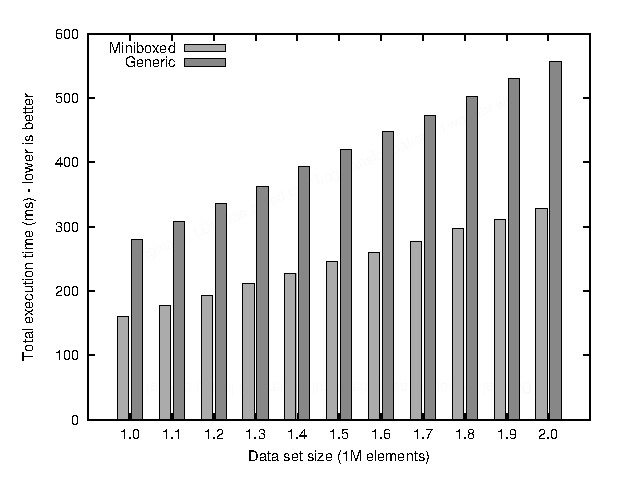
\includegraphics[width=0.45\textwidth]{graph.eps}
\caption{Least squares method using linked lists}
\label{fig:linkedlist}
\vspace{-1.0em}
\end{figure}

\textbf{Runtime performance.} Since the miniboxing plugin has been around for some time, its runtime performance has been thoroughly benchmarked \cite{miniboxing}. The most recent result is a benchmark on a slice of the Scala collections library \cite{miniboxing-linkedlist} centered around the linked list collection. The benchmark consists of running the least squares method for fitting data points on several input sizes. The results, summarized in Figure \ref{fig:linkedlist}, show a 45\% speedup produced by using the miniboxing transformation. It should be noted that Scala collections are notoriously hard to transform, since they use many advanced features of the language, such as type classes, higher-kinded types and anonymous and nested classes. Indeed, we also tried to run the benchmark with the current specialization transformation in the Scala compiler \cite{iuli-thesis}, but the results were disappointing: due to technical difficulties, the specialized linked list was slower than the generic one.

The miniboxing plugin \cite{miniboxing-www} has also transformed larger projects, with spire \cite{erik-spire} being the largest at 31KLoC, and produced reliable results. This shows the LDL mechanism is not just a toy but can correctly transform large code bases.

\textbf{Two extra features} are added by the miniboxing plugin over the standard LDL mechanism:
\begin{itemize}
\item using multiple alternative representations, |Long| and |Double| in the current version. To implement this, the |@storage| annotation was parameterized with a type, allowing the \inject{} phase to include the target representation in the annotation: |@storage[Long]| $\rightarrow$ |Long| and |@storage[Double]| $\rightarrow$ |Double|. This lead to a third coercion marker, |marker_minibox2minibox|;
\item a second LDL cycle is used to change the object-oriented representation of functions to a miniboxing-friendly representation.
\end{itemize}
These additions are described on the miniboxing website \cite{miniboxing-www}.

\subsection{Case Study 3: Staging}
\label{sec:validation/staging}
Multi stage programming \cite{taha-intro} allows a program to execute in several steps, at each step generating new code, compiling and then executing it. In Scala, this technique has been used by \textem{Rompf} to develop the lightweight modular staging (LMS) framework \cite{tiark-lms, tiark-building-blocks}, which removes the cost of abstraction in many high-level embedded DSLs \cite{tiark-thesis, staged-sac, nada-js,stucki-odds,ackermann-jet}.

Using the LMS framework requires the ability to lift built-in language constructs, such as method calls, |if| expressions and variable accesses. This is done by transforming these constructs into calls to methods provided by the programmer or by the LMS framework. Currently, lifting is done using a custom version of the compiler, dubbed scala-virtualized \cite{scala-virtualized} or using Yin-Yang \cite{yin-yang}, a macro-based frontend that allows selectively lifting parts of a program.

In this section, we show that lifting can be modelled as a data representation transformation, allowing LDL-transformed programs to be optimized by an LMS-like framework. One of the early examples of staging given by \textem{Rompf} is eliminating the recursion from a power function:

\begin{lstlisting-nobreak}
 def pow(b: `@staged` Double, e: Int): `@staged` Double =
   if (e == 0) 1.0
   else if (e % 2 == 1) b * pow(b, e-1)
   else {
     val x = pow(b, e/2)
     x * x
   }
 val pow5 = function(arg => pow(arg, 5))
 println("3.0^5 = " + pow5(3.0))
 println("4.0^5 = " + pow5(4.0))
\end{lstlisting-nobreak}

The |pow| method computes $\texttt{b}^{\texttt{e}}$. The base, |b|, and the return type are marked as |@staged|, whereas the exponent, |e|, is not. This means that calls to |pow|, instead of computing a value, accumulate the operations necessary to produce $\texttt{b}^{\texttt{e}}$ for a variable base |b| and a fixed exponent |e|.


Indeed, the call to |function| in line 8 first triggers the execution of |pow| for the variable base |b=arg| and the fixed exponent |e=5|. The operation graph recorded corresponds to $\texttt{arg}^{\texttt{5}}$ and is used by the |function| call to generate optimized code, compile it, and to expose it as a function from |Double| to |Double|, corresponding to $\texttt{arg => arg}^\texttt{5}$:

\begin{lstlisting-nobreak}
 function: compiling the following code:
 ***************************************
   (arg: Double) => {
     val x0: Double = arg * arg
     val x1: Double = x0 * x0
     val x2: Double = arg * x1
     x2: Double
   }
 ***************************************
 3.0^5 = 243.0
 4.0^5 = 1024.0
\end{lstlisting-nobreak}

The generated code shows the |if| conditional and the recursive calls were eliminated. Indeed, running |pow| for the exponent |5| executes exactly three non-trivial operations transitively involving the argument |arg|, all three appearing in the generated code. This shows the operations were lifted and recorded in the operation graph, allowing the code above to be generated in the next stage. Let us see how the |pow| code was transformed to allow lifting.

In the case of staging, there is \textbf{no \inject{} phase}, since the programmer manually marks the arguments to be |@staged|.

\textbf{The \coerce{} phase} follows the usual pattern of introducing coercions, with an additional constraint: immediate values can be coerced to staged constants, but not the other way around. This is done so that staging and compiling are only triggered explicitly, through calls such as |compile| and |function|. This restriction could easily be removed, but keeping it makes the performance predictable, as it puts the programmer in control of the lengthy staging and compilation process. Seen in relation to primitive types, when staging, boxing is cheap, but unboxing can potentially be expensive, so we want to trigger it explicitly.

The \coerce{} phase is also responsible for redirecting method calls for |@staged| receivers, which is essentially the lifting mechanism. Unlike the previous transformations, where extension methods were either provided by the library or extracted automatically, in the case of staging, they are manually written by the programmers. These methods are called infix methods \cite{scala-virtualized} and they contain the mechanism to build the operation graph used to generate optimized code. Since this part is very similar to what is done in the LMS framework and is not our contribution, we point the reader to the works of \textem{Rompf} \cite{tiark-lms, tiark-building-blocks, tiark-thesis} for more details.

%  - The commit phase commits to the staged representation and rewires method calls
\textbf{The \commit{} phase} transforms |@staged T| to the operation graph representation used in LMS, |Rep[T]|, and redirects calls to |compile| and |function| to |compile_impl| and |function_impl|, which trigger the synthesis and compilation for the operation graph.

The staging prototype serves to show that lifting language constructs can be modelled as an LDL-based representation transformation.

\subsubsection{Evaluation}

\textbf{Lines of code and complexity.} The staging plugin consists of 12 Scala files with 487 lines of code. The difference between the standard Scala compiler and Scala-virtualized is +2247/-578 LOC, including the library changes necessary to support lifting language constructs. Although the staging plugin is still far from being on-par with scala-virtualized in terms of lifting capabilities, it is 4 times smaller, despite the boilerplate necessary to create a Scala compiler plugin.

The \commit{} phase for the staging plugin has 110 lines of code and 5 transformation rules:
\begin{itemize}
\item  3 rules for redirecting markers to actual coercions;
\item  2 rules for the special methods |compile| and |function|.
\end{itemize}

\textbf{Runtime performance.} We tested the staging plugin on the FFT example from Rosetta Code \cite{rosetta-code}. To stage the FFT example, we lifted the operations on complex numbers but left everything else to evaluate during staging. The separation into even and odd numbers and all the butterfly connections specific to FFTs are done only once during staging. Of course, this requires deciding on the number of elements ahead of time, thus fixing the batch size for the FFT analysis. With this, we get the following results:

\begin{lstlisting-nobreak}
 ::Benchmark FFT.Scala Complex::
 Parameters(data size = 2^ -> 3): 0.966099

 ::Benchmark FFT.Stagium Complex::
 Parameters(data size = 2^ -> 3): 0.018612
\end{lstlisting-nobreak}

The times for executing the FFT (expressed in milliseconds) suggest that lifting the code and removing collection-related abstraction can bring a speedup of 53x, making staging worth it when running the FFT code multiple times.

\textbf{The two extra features} in the staging plugin are: (1) using programmer-written infix methods instead of synthetic or library extension methods and (2) the ability to restrict a class of coercions, in this case from staged to direct values, outputting meaningful error messages and explaining the problem to the user.

\section{Related Work}
\label{sec:related}

\textbf{Generics.} Interoperation with generics motivates many of the data representation transformations in use today. The implementation of generics is influenced by two distinct choices: the choice of low-level code translation and the runtime type information stored.

The low-level code generated for generics can be either heterogeneous, meaning different copies of the code exist for different incoming argument types or homogeneous, meaning a single copy of the code handles all incoming argument types. Heterogeneous translations include Scala specialization \cite{iuli-thesis}, compile-time C++ template expansion \cite{cxx-stroustrup} and load-time template instantiation \cite{dot-net-generics} as done by the .NET CLR \cite{ecma-dotnet}. Homogeneous translations, on the other hand, require a uniform data representation, which may be either boxed values \cite{java-erasure, leroy-unboxed-objects}, fixnums \cite{fixnums-lisp} or tagged unions \cite{morrison-napier88}.

In order to perform tests such as checking if a value is a list of integers at runtime, the type parameter must be taken into account. In homogeneous and load-time template expansions, one has to carry reified types for the type parameters. While this has an associated runtime cost \cite{michel-thesis}, several solutions have been proposed to reduce it: in the CLR, reified types are computed lazily \cite{dot-net-generics}. In Java, several papers presented viable schemes for carrying reified types, including PolyJ \cite{myers-polyj}, Pizza \cite{pizza}, NextGen \cite{cartwright-nextgen} and the work by \textem{Viroli et al.} \cite{viroli-reflective}. Finally, in ML, generic code (also called parametrically polymorphic in functional languages) can carry explicit type representations \cite{harper-intensional-type-analysis, tarditi-til}.

\textbf{Unboxed primitive types.} In the area of unboxed primitive types, \textem{Leroy} \cite{leroy-unboxed-objects} presents a formal data representation transformation for the ML programming language based on typing derivations. The comparison in the introduction states that Late Data Layout introduces selectivity, object-oriented support and disentangles the transformation from its assumptions. This is a somewhat shallow comparison. A deeper comparison is that in \textem{Leroy}'s transformation the \inject{} and \commit{} phases are implicit and hard-coded while the two versions of the transformation rules presented by \textem{Leroy} correspond to duplicating the \coerce{} phase for boxed and unboxed expected types. Instead of expected types, the ML transformation knows where generic parameters occur, and uses this information to invoke the correct version of the transformation. Therefore our main contribution is discovering and formulating the underlying principle and successfully extending it to a more broad context, to include value classes, specialization and staging, which have very different requirements.

\textem{Shao} further extends \textem{Leroy}'s work \cite{shao-compiler-ml, shao-flexible-representation-analysis} by presenting a more efficient representation, at the expense of carrying explicit type representations \cite{harper-intensional-type-analysis, tarditi-til}. \textem{Minamide} further refines the transformation and is able to formally prove that the transformed code has the same time complexity as the original program \cite{minamide-unboxing-runtime-complexity}. Tracking value representation in types has been presented and extended to continuation-passing style \cite{flanagan-essence-cps} by \textem{Thiemann} in \cite{thiemann-unboxed-objects-cps}. Two pieces of information are tracked in a lattice: whether the value corresponding to the type is used at all (otherwise its representation can be ignored - called ``Don't care polymorphism'' and equivalent to our |oblivious| relation between AST nodes) and whether a certain representation is required. This information is used in a type inference algorithm which can elide coercions when the parameters are discarded or when a method call is in tail position, namely it doesn't need to box the result only to have the caller unbox it. It should be noted that the coercions operate on a continuation-passing-style intermediary representation.

A different direction in unboxing primitive types is based on escape analysis \cite{escape-analysis-first-paper}, where the program is analyzed at runtime and a local and conservative data representation transformation is performed. When implemented in just-in-time compilers \cite{stadler-escape-analysis} of virtual machines such as PyPy \cite{bolz-pypy-tracing-jit}, Graal \cite{graal} or HotSpot \cite{hotspot-c2}, and coupled with aggressive inlining, the escape analysis can make an important difference, although it is limited by not being able to optimize containers outside its local scope. Late Data Layout and escape analysis are fundamentally different -- escape analysis has a local scope and relies heavily on inlining, while LDL can safely optimize across method boundaries as long as the transformation consistently makes the same decisions in subsequent separate compilations. Interpreter-based techniques such as quickening \cite{quickening} and trace-based specialization \cite{tracemonkey} can further improve escape analysis based on the dynamic execution profiles. Truffle \cite{truffle} partially evaluates the interpreter for the running program and makes aggressive assumptions about the data representation, yielding the best results in terms of top speed at the expense of a longer warm-up time.

The Haskell programming language has two reasons to box primitive types in the low level code: (1) due to the non-strictness of the language, arguments to a function may not have been evaluated yet and are thus represented as thunks and (2) due to erased parametric polymorphism. Haskell exposes both the boxed |Int| representation and the unboxed |Int#|, although the compiler does transform |Int| values to |Int#| where possible. To do so, the Glasgow Haskell Compiler uses a syntax-based transformation coupled with a peephole optimization \cite{spj-unboxed-values, launchbury-unpointed}. In general, peephole optimizations have been formalized by \textem{Henglein} in \cite{henglein-formally-optimal-boxing}. Haskell also features calling convention optimizations that make the argument laziness explicit and can unbox primitives in certain situations \cite{bolingbroke-haskell-calling-conventions}.

\textbf{Value classes} have been proposed for Java as early as 1999 \cite{gosling-value-classes, rose-value-classes-vm, rose-value-classes-tearing}. The most recent description, which is also closest to our current approach, is the value class proposal for the Scala programming language \cite{scala-value-classes-sip}. We build upon the idea that a single concept should be exposed despite having multiple representations, but we step away from ad-hoc encodings and fixed rules in the type system. In this way, we can capture other representations, such as the tagged representation in \cite{morrison-napier88}. Value classes have also been implemented in the CLR \cite{dot-net-value-types-www}, but to the best of our knowledge the implementation has not been described in an academic setting. The Haskell programming language offers the |newtype| declaration \cite{haskell-newtype} that, modulo the bottom type $\bot$, is unboxed similarly to value classes.

\textbf{Specialization} for generics is a technique aimed at eliminating boxing deep inside generic classes. Specialization has been implemented in Scala \cite{iuli-thesis, specialization-iuli} and has been improved by miniboxing \cite{miniboxing, miniboxing-www}. Specialization and macros have been combined to produce a mechanism for ad-hoc specialization of code in Scala \cite{bridging}. The .NET CLR automatically specializes all generics, thanks to its bytecode metadata and reified types \cite{dot-net-generics}.

A different approach to deep boxing elimination is described for Haskell \cite{spj-dph} and Python \cite{bolz-python-strategies}. It relies on specializing arrays while providing generic wrappers around them. This allows memory-efficient storage without the complex problem of providing heterogeneous translations for each of the methods exposed by data structures.

\textbf{Multi-stage programming} (also called staging) \cite{taha-intro} requires lifting certain expressions in the program to a reified representation. Staging can be implemented using macros \cite{taha-macroml, eugene-macros, yin-yang}, or using specialized compiler extensions \cite{scala-virtualized}. One of the applications is removing the abstraction overhead of high-level and embedded domain specific languages. Indeed, staging was successfully used to optimize and re-target domain-specific languages (DSLs) \cite{tiark-thesis, tiark-lms, tiark-building-blocks, delite, nada-js, staged-sac}.

\textbf{Annotated types} \cite{sip-annotations, jsr-annotations} have been introduced to trigger code transformations and to allow the extension of the type system into the area of program verification while reusing as much infrastructure from the compiler as possible \cite{papi-annot-typechecker}. In the context of Java, type annotations have been used to selectively add reified type argument information to erased generics \cite{prodromos-refied-type-args}. In the context of Scala, annotated types have been used to track and limit the side-effects of expressions \cite{lukas-effects-ecoop, lukas-thesis}, to designate macro expansions \cite{eugene-macros} and to trigger continuation-passing-style transformations \cite{tiark-cps}.

\textbf{Formalization.} In \cite{leroy-unboxed-objects}, \textem{Leroy} presents a full formalization for the primitive unboxing for ML, including a proof of operational equivalence. The .NET generics are formalized in \cite{dot-net-generics-form}. An effort to formalize LDL is currently on-going \cite{ldl-form} and it relies on local type inference, as described by \textem{Odersky et al.} \cite{odersky-colored-local-type-inf} and \textem{Pierce et al.} \cite{pierce-local-type-inference}.

In the area of formal descriptions, two papers on type-directed coercion insertion stand out as very closely related to this paper \cite{swamy-typed-coercions, leather-type-changing-rewriting}. The work of {\em Swami} et al. \cite{swamy-typed-coercions} focuses on automatically composing several coercions together in order to bridge the gap between different types. The highlight of the paper are the powerful composition rules and the proofs that, despite their generality, always produce syntactically unique, non-ambiguous rewritings. This work resembles the mechanisms used to introduce implicit conversions in Scala, although the rules provide more flexibility and are proven not to diverge. On the other hand, {\em Leather} et al. \cite{leather-type-changing-rewriting} describe a coercion insertion mechanism which deliberately produces ambiguous rewritings from which heuristics can pick the best. More importantly, the formalism presented in \cite{leather-type-changing-rewriting} is also capable of consistently changing types in the rewrite rules, making the transformation very versatile. Unfortunately, the two formalisms do not handle backward propagation, object orientation and subtyping, all of which are crucial to performing optimal data representation transformations in Scala. Furthermore, they do not provide the ability to selectively transform the data representation, making them unusable for the three use cases we presented. By comparison, an important limitation of our work is that the |box| and |unbox| coercions we introduce are un-ambiguous and not composible by design, as we aim for a one-step conversion between different representations.

\section{Acknowledgements}

We would like to thank Aymeric Gen\^et, who developed the least squares benchmark for the miniboxing plugin \cite{miniboxing-linkedlist}.

We are grateful to the Scala teams at EPFL and Typesafe for providing precious feedback and helping shape the representation mechanism we have today. In particular, we would like to thank Manohar Jonnalagedda, Dmitry Petrashko, Iulian Dragos, Miguel Garcia and Lukas Rytz for the discussions we had, which always led to interesting developments. We are thankful to the Scala community, for trying the project, reporting bugs and providing cool new ideas. We would like to thank our paper and artifact reviewers in the OOPSLA conference for providing clear and concise feedback, which guided us in improving the paper.

Last but not least, Vlad is grateful to his wife Ana Lucia and his family who supported him through very difficult times when this paper was written. \iv{Vă pup!}

\section{Conclusion}

In this paper we presented a general mechanism that allows refining a high-level concept into multiple representations. This is done in a selective way, by annotating  values in the program with their desired representation. The coercions necessary for maintaining program consistency with regards to representations are introduced automatically, consistently and optimally thanks to local type inference.

We validated the algorithm for three cases: multi-pa\-ram\-e\-ter value classes, specialization through miniboxing and a simple multi-stage programming mechanism. The results were encouraging: we were able to reuse much of the infrastructure (which has been developed as part of the miniboxing plugin) for the other plugins and the development time was in the order of developer-weeks.

Finally, the key insights of the paper are that annotated types are a perfect vehicle for carrying representation information and introducing coercions can be done consistently and optimally using the expected type mechanism in local type inference.

